%%%%%%%%%%%%%%%%%%%%%%%%%%%%%%%%%%%
%% Setup
%%%%%%%%%%%%%%%%%%%%%%%%%%%%%%%%%%%

\glsresetall
\glsunset{H2O}

% Create a row in a table that references the documentation.
\DeclareDocumentCommand\docrow{mom}{% mandatory (m), optional (o), mandatory (m)
  \ifthenelse{\equal{#2}{\NoValue}}{%
    \hspace{0.9em}\labelitemi\hspace{1.0\itemsep}\ref{#1} & \hyperref[#1]{\modelica{#3}} \\
  }{%
    \hspace{0.9em}\labelitemi\hspace{1.0\itemsep}\ref{#1}--\ref{#2} & \modelica{#3} \\
  }
}

% Trim and frame GUI images.
\DeclareDocumentCommand\gui{om}{% optional (o), mandatory (m)
  \ifthenelse{\equal{#1}{\NoValue}}{%
    \fbox{\lwincludegraphics[clip, trim=6 6 6 23.5]{#2}}
  }{%
    \fbox{\lwincludegraphics[clip, trim=6 6 6 23.5, #1]{#2}}
  }%
}%

% Border for GUI images
\setlength\fboxsep{0pt}
\setlength\fboxrule{0.5pt}

%%%%%%%%%%%%%%%%%%%%%%%%%%%%%%%%%%%
%% Content
%%%%%%%%%%%%%%%%%%%%%%%%%%%%%%%%%%%
 
% \begin{singlespaced}
%   \epigraph{``The idea that terminal variables can be divided into efforts and flows appears to be a deep---but unfortunately largely unexplored---physical principle, corroborated by many examples.''}{Jan Willems~\cite{Willems2007}}
% \end{singlespaced}

This chapter describes how the model is implemented in the Modelica language~\cite{Modelica3.3}.  It serves primarily as a summary for \autoref{chap:Doc}, which contains documentation generated from the source code.  The documentation contains auto-generated tables, diagrams, and code listings.  It also contains discussions and other details such as lists of assumptions which have been manually written and embedded using Modelica's annotations.  That information is only referenced here to avoid redundancy.

The introduction below merely sets the context to describe the model library.  For an introduction to the Modelica language, see~\cite{Tiller2002} or~\cite{ModelicaTutorial1.4}.


\section{Introduction}

The models are special object-oriented classes in the Modelica language.  The model library also uses other classes such as connectors, blocks, functions, records, packages, types.  The classes are encapsulated and organized hierarchically via inheritance and instantiation.  Encapsulation or abstraction hides details about the implementation, leaving only the meaningful characteristics accessible from outside the class~\cite{Pyster2012}. %[p. 91]
Inheritance creates models or other classes by extending or adding to more general and basic classes.  It helps to organize the library and reduce the amount of duplication in the code.  Instantiation allows classes to be built by assembling working copies of lower-level classes.  This is consistent with the physical hierarchy of the fuel cell (e.g., a cell is an assembly of layers).  \autoref{fig:ModelHierarchy2} shows that the model is created by instantiating species into phases, phases into subregions, subregions into regions such as a fuel cell layer, and regions into assemblies such as a fuel cell.  By convention, the names of classes begin with an uppercase letter and their instances start with a lowercase letter.  Subclasses and sub-instances are accessed via dot notation (e.g., \modelica{Class.Subclass1.Subclass2}).


\begin{figure}[htbp]
  \newcommand{\I}[1]{\fbox{\includegraphics[height=2cm]{#1}}}
  \newcommand{\arrow}{\vbox to 1.95cm {\vfil
    \hbox{\LARGE $\rightarrow$}
    \vfil}}
  \I{4-SpeciesI}~\arrow~\I{4-PhaseI}~\arrow~\I{4-SubregionI}~\arrow~\fbox{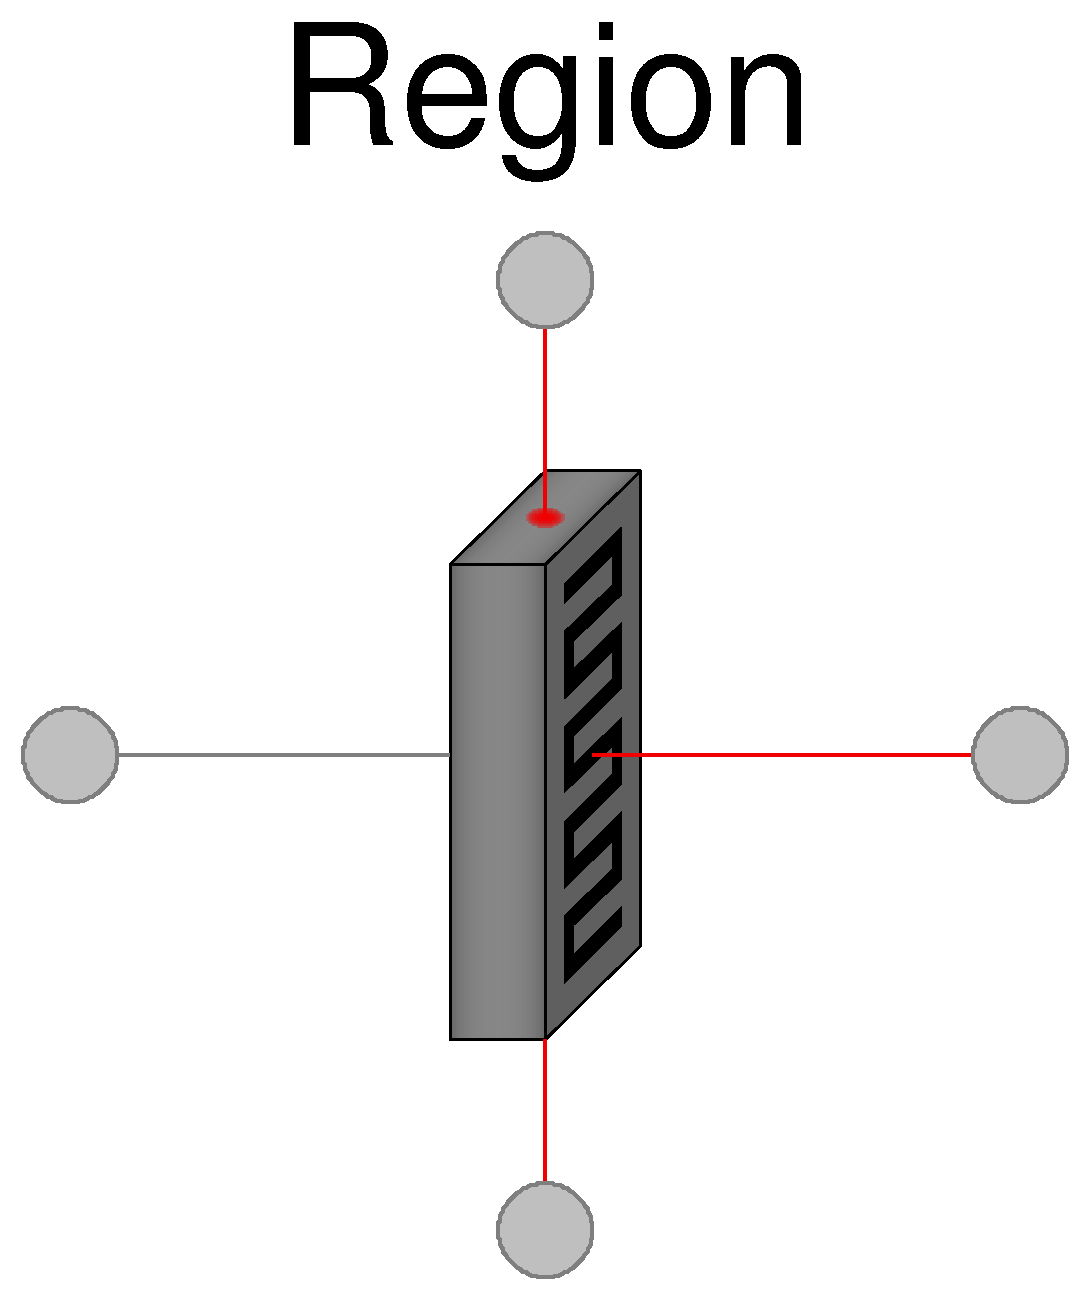
\includegraphics[height=2.4cm]{4-RegionI}}~\arrow~\I{4-AssemblyI}%
  \caption{Levels of instantiation in the model library (duplicate of \autoref{fig:ModelHierarchy})}%
  \label{fig:ModelHierarchy2}%
\end{figure}


Each model is a system with possible subsystems.  The physical connectors (i.e., connectors containing efforts and flows, to be discussed later) of the model represent its boundaries.  The boundaries may be geometric (e.g., the positive boundary along the x axis; see \autoref{fig:Flow3DLabel}) or conceptual (e.g., between two species within a phase).

The equations of a model may be represented graphically or textually.  Usually, the higher-level models are graphical whereas the lower-level ones are textual.  In the diagrams, lines between physical connectors (\autoref{sec:Connectors}) comprise nodes which are subject to the generalized Kirchhoff circuit laws (e.g., efforts are equal and flows sum to zero).  The icons represent instances of classes.

The term \emph{\n{state}} should be clearly defined because it has two different (but related) meanings in mathematical modeling and thermodynamics.  In the context of modeling and Modelica\glsadd{state-model}, a state is a scalar time-varying variable of which a derivative is taken.\footnote{These may or may not be the same variables which are wrapped by the \modelica{der()} operator since the Modelica translator is usually free to choose appropriate states.  Also, those variables may be algebraically coupled, in which case the translator must perform index reduction.}  The states of a model are necessary and sufficient to determine the values of all other variables of the model at a given time.  In the context of thermodynamics\glsadd{state-thermo}, a state is the condition of a system.  It encompasses a set of properties with cardinality equal to the degrees of freedom of the system in the sense of Gibbs' phase rule~\cite{Moran2004, Bejan2006}.  Since the fuel cell models involve thermodynamics, both meanings may be used.  A thermodynamic state is represented by a set of model states---generally one for each mode of energy storage (e.g., pressure and temperature).

The remaining sections describe the model library from low to high level.  The first sections describe supporting classes such as types (\autoref{sec:Quantities}), constants (\autoref{sec:Units}), records and functions (\autoref{sec:Characteristics}), and connectors (\autoref{sec:Connectors}).  The models begin with the subregions in \autoref{sec:Subregions} and continue up to the test models in \autoref{sec:TestStand}.


\section{Quantities}
\label{sec:Quantities}

\begin{contextbox}
  Related section of the documentation:
  \vspace{0.5\baselineskip}

  \renewcommand{\arraystretch}{1.5}
  \begin{tabular}{ll}
    \docrow{sec:FCSys_Quantities}{FCSys.Quantities}
  \end{tabular}
\end{contextbox}

Quantities are types used to represent physical values in the model library.  Each quantity has a dimension which is specified in terms of angle (A), length (L), mass (M), particle number (N), and time (T).  Quantities may also have default display units and minimum or maximum values.

Instances of quantities are variables.  The names of the variables match those in \autoref{chap:Fundamentals} with the exceptions that \begin{inparaenum}[(1)]\item Greek letters are spelled in English and \item subscripts begin with an underscore\end{inparaenum}.  Usually, extensive properties are uppercase and intensive properties are lowercase.

The quantities package is described further in the documentation (\autoref{sec:FCSys_Quantities}).  Throughout the rest of this chapter and the appendix, the \modelica{Quantities} package may be abbreviated as \modelica{Q} (e.g., \modelica{Q.Length}).


\section{Units}
\label{sec:Units}

\begin{contextbox}
  Related sections of the documentation:
  \vspace{0.5\baselineskip}

  \renewcommand{\arraystretch}{1.5}
  \begin{tabular}{ll}
    \docrow{sec:FCSys_Units}{FCSys.Units}
    \docrow{sec:FCSys_Units_Bases}[sec:FCSys_Units_Bases_Base]{FCSys.Units.*}
  \end{tabular}
\end{contextbox}

The \modelica{Units} package is described in \autoref{sec:FCSys_Units} with updated information from the related paper~\cite{Davies2012ModelicaUnits}.  In summary, the approach is based on the concept that a quantity is the product of a number and a unit~\cite{BIPM2006}.  The variables in the library represent quantities,  in contrast to the usual approach where variables represent numbers or quantities expressed in a unit (where ``expressed in'' means divided by).  When a variable is given a quantity in the library, it is expressed literally as the product of a number and a unit or group of units.  This provides convenience and flexibility in entering values (e.g., \modelica{101325*Pa} or \modelica{1*atm}).  When the variable is expressed in a unit, it is divided by that unit (e.g., \modelica{p/kPa}).

The units package begins by giving values to certain fundamental, physical, and measurable constants (the speed of light in vacuum and the Rydberg, Josephson, von Klitzing, Faraday, and gas constants).\footnote{The radian and candela are also given values to complete the basis.  As discussed, the radian must be one due to the definition in~\cite{BIPM2006}.}  The values are arbitrary except that they can be used to additionally scale the floating point variables.  The units are then determined by the accepted values of the constants (e.g., $c = \SI{299792458}{m/s}$ from~\cite{NIST2010}).  The constants have independent dimensions such that they are sufficient to determine the values of all other units.  Approximately 90 constants, units, and prefixes are defined.  All are instances of quantities (as defined in \autoref{sec:Quantities}).

As noted in the beginning of \autoref{chap:Fundamentals}, the model equations are written in a system of units where the Faraday and gas are normalized to one.  Literally, this means that $\SI{1}{mol} = \SI{96485.3365}{C}$.  The coulomb is used as a number of particles just as the mole, but the charge number is applied appropriately when describing an electric field or an electric current.  Since the Faraday and gas constants are both normalized, temperature is equivalent to thermal voltage (e.g., $\SI{300}{K} \approx \SI{25.85}{mV}$).  This also implies that the Boltzmann constant is normalized to \s{q}, the particle number representing a single particle.  These normalizations simplify the equations and make it straightforward to model electrons and protons like other species (albeit with nonzero charge number).

During the implementation, it was discovered that the document which establishes the International System of Units (SI)\glsunset{SI}~\cite{BIPM2006} may inconsistently define and use angles.  Table~3 in that document states that the radian (rad) is defined by $\si{rad} \equiv 1$ and the hertz (Hz) is defined by $\si{Hz} \equiv \si{s^{-1}}$.  However, we commonly consider the hertz to be a measure of ``cycles per second'' or $\si{Hz} = \si{cyc}/\si{s}$, where the cycle (cyc) is defined by $\si{cyc} \equiv \SI{2\pi}{rad}$ in trigonometry.  Since $\si{rad} \equiv 1$, it follows that $\si{cyc} = 2\pi$.  This implies that $\si{Hz} = 2\pi/\si{s}$, which is not consistent with the \n{SI} definition ($\si{Hz} \equiv \si{s^{-1}}$).

The discrepancy could be resolved by defining angle as an explicit dimension (like length and time) with units that include the radian, cycle, and degree.  Those units are related (e.g., $\si{cyc} \equiv \SI{2\pi}{rad}$) but none should be given a fixed value.  That is the approach in the \modelica{Units} package, but it is limited by the fixed \n{SI} definition of $\si{rad} \equiv 1$.  The approach also resolves issues such as the seemingly identical units of energy (\si{J}) and torque (\si{N.m})~\cite{McNish1957} by using angle in the units for torque (e.g., $\si{J/rad}$).  In this sense, torque is a unit of energy per swept angle.  Traditionally, we express the angle in radians but exclude it (since it is one) and then consider torque to be the product of force and radius.

Throughout the rest of this chapter and the appendix, the \modelica{Units} package may be abbreviated as \modelica{U}.  For example, \modelica{U.m} is the unit meter.


\section{Characteristics}
\label{sec:Characteristics}

\begin{contextbox}
  Related sections of the documentation:
  \vspace{0.5\baselineskip}

  \renewcommand{\arraystretch}{1.5}
  \begin{tabular}{ll}
    \docrow{sec:FCSys_Characteristics_BaseClasses_Characteristic}[sec:FCSys_Characteristics_O2_Gas]{FCSys.Characteristics.*}
  \end{tabular}
\end{contextbox}

The \modelica{Characteristics} package contains data and functions to correlate physical properties of materials.  The data and functions are contained within a package for each chemical species.  All of the correlated and derived thermodynamic properties (Sections~\ref{sec:CorrelatedThermo} and \ref{sec:DerivedThermo}) and diffusion properties (Sections~\ref{sec:Exchange} and \ref{sec:Transport}) are coded from the descriptions in the previous chapter.  The characteristics are suitable for real and ideal gases, compressible and incompressible fluids, and solids.  \autoref{tab:FCSys_Characteristics_BaseClasses_Characteristic-contents} lists the data and functions.

The Modelica media package (\modelica{Modelica.Media}~\cite{ModelicaSL3.2}) is not used besides its data.  There are four reasons.  First, it would be necessary to rewrite the variable declarations since the model library uses a different approach to physical units (see the previous section).  Second, many of the functions would need to be wrapped to convert the properties for the equations established in \autoref{chap:Fundamentals}.  This would introduce overhead in terms of both computation and software maintenance.  Third, some properties are not available in \modelica{Modelica.Media}.  Other properties and correlations are present but are not needed.  Finally, the models are factored differently in the present library.  The \modelica{Characteristics} package does not include any models or time-varying variables (in the \modelica{Species} model instead---next section), unlike \modelica{Modelica.Media}.

The virial coefficients (\s{p}-\s{v}-\s{T} relation) for the Leiden (volume-explicit) form are encoded in a matrix (\s{b}[_v]).  The power of $\s{p}/\s{T}$ increases by row and the power of~\s{T} increases by column, beginning with the powers set by~\s{n}[_v] (a 2-tuple).  The matrix for the Berlin (pressure-explicit) form (\s{b}[_p]) is computed automatically but is currently limited to the fourth virial coefficient.  It can be expanded to an arbitrary order with results from a \n{CDF} file included with the library.  The Leiden is directly prescribed instead of the Berlin form so that the specific volume of incompressible species can be entered.  The resulting polynomials are encoded in all the property functions using the nested form (e.g., $f(x) = ((\ldots + a_\text{-1-n})/x + a_\text{-n})/x + a_\text{1-n} + x\cdot(a_\text{2-n} + x\cdot(a_\text{3-n} + \ldots))$) for computational efficiency.

The isobaric specific heat capacity-temperature relation also allows arbitrary polynomial order, starting from an arbitrary power.  This makes it possible to prescribe constant or temperature-dependent specific heat capacity as needed.  The relation is independent of pressure, but following the approach by Dymond et al.~\cite{Dymond2002}, the rows of the coefficients matrix (\s{b}[_c]) cover different temperature ranges.  An arbitrary number of rows can be included, which is an improvement over \modelica{Modelica.Media}.

A base characteristics record is extended for each of the chemical species required for the fuel cell model---\n{C+}, negatively charged Nafion sulfonate (\s{C19HF37O5S-}, abbreviated as \s{SO3-}), \n{e-}, \n{H+}, \n{H2}, water vapor, liquid water, water absorbed in the ionomer, \n{N2}, and \n{O2}.  Where available, virial and heat capacity coefficients are included respectively from~\cite{Dymond2002} and~\cite{McBride2002} (directly or via \modelica{Modelica.Media}).  These representations are later simplified (e.g., to ideal gas and constant specific heat capacity) as appropriate.   The polynomial coefficients for the specific heat capacity of water in the ionomer and the associated integration constants for enthalpy and entropy are set so that the hydration of the ionomer matches the correlation of Springer et al.~\cite{Springer1991} at 0 and 100\% relative humidity.  For simplicity, the model is not matched to that correlation over the full range of relative humidity.


\section{Connectors}
\label{sec:Connectors}

\begin{contextbox}
  Related sections of the documentation:
  \vspace{0.5\baselineskip}

  \renewcommand{\arraystretch}{1.5}
  \begin{tabular}{ll}
    \docrow{sec:FCSys_Connectors}{FCSys.Connectors}
    \docrow{sec:FCSys_Connectors_Amagat}[sec:FCSys_Connectors_Translational]{FCSys.Connectors.*}
  \end{tabular}
\end{contextbox}

Interactions between physical models are described by connections involving pairs of flow and effort variables.  The flow variable (or simply ``flow'') is typically the rate at which a conserved quantity enters a control volume through the associated interface.  The effort variable (or ``effort'') is typically a property which drives diffusion of the quantity.  When connectors are joined, a node is formed where the sum of the flows is zero~\cite{West2001} %\cite[p. 176]{West2001}
(e.g., \nname{KCL}) and the efforts are equal (e.g., \nname{KVL})~\cite{Thomas1998, Willems2010}.  The essence is that connected systems experience the same value of a property at their shared boundary, and when a quantity leaves one system, it immediately enters another (the quantity is not created, destroyed, or stored in the node).

\autoref{tab:Connectors} lists the effort\slash{}flow pairs of the physical connectors in the model library.  The material pair transfers material between regions.  Its flow, \dot{N}, is the current or flow rate of material.  The pressure, \s{p}, is the thermodynamic pressure. The translational pair transports or exchanges translational momentum due to drag between regions or among species within a region.  It is similar to the Modelica mechanical translational connectors (e.g., \modelica{Modelica.Mechanics.Translational.Interfaces.Flange_a}) except that the effort is velocity rather than position.  The reason is that Modelica mechanics is Lagrangian (i.e., consisting of control masses) whereas the fuel cell model library is Eulerian (i.e., consisting of control volumes).  The thermal advective pair exchanges thermal energy between reactants and products in a chemical reaction.  The thermal diffusive pair transports or exchanges heat due to thermal conduction between regions or species within a region.  It is similar to \modelica{Modelica.Thermal.HeatTransfer.Interfaces.HeatPort}.  The thermodynamic state is defined at a boundary through temperature and pressure; therefore, $\s{s}\s{T}$~is known and thermal advection can be determined.  The Amagat pair adds the volumes of phases that exist at a certain pressure within a region.  The Dalton pair is the opposite; it adds the pressures of species that exist within the volume of a phase.  The chemical pair is used for phase change and for the connections leading up to a reaction where material is conserved without reaction.  The stoichiometric pair is its opposite.  It is used to add the stoichiometrically-weighted chemical potentials of the species involved in a chemical reaction.  Its effort is the rate of the reaction, which is common to all of the connected species.

\begin{sidewaystable}[hbtp]
  \caption{Effort\slash{}flow pairs of the connectors}
  \label{tab:Connectors}
  \newcommand\C[1]{\multirow{1}*{#1}} % Hack to vertically align entries in a table
\newcommand\G[1]{\C{\includegraphics[height=1cm]{#1}}} % Insert a graphic across two rows.
\begin{tabular}{llll}
  \toprule
  \textbf{Name} & \textbf{Effort} & \textbf{Flow} & \textbf{Within icon(s)} \\
  \midrule \addlinespace
  \C{Material} & Pressure & Current & \G{4-Connectors-BoundaryI}\G{4-Connectors-BoundaryBusI} \\
    & \s{p} [\dim{M.L^{-1}.T^{-2}}] & $\dot{N}$ [\dim{N.T^{-1}}] \\ \addlinespace
  \C{Translational} & Velocity & Force & \G{4-Connectors-BoundaryI}\G{4-Connectors-BoundaryBusI}\G{4-Connectors-IntraI}\G{4-Connectors-InterI}\G{4-Connectors-ReactionI} \\
    & \s{phi} [\dim{L.T^{-1}}] & $\dot{mPhi}$ [\dim{L.M.T^{-2}}] \\ \addlinespace
  \C{Thermal diffusive} & Temperature & Heat flow rate & \G{4-Connectors-BoundaryI}\G{4-Connectors-BoundaryBusI}\G{4-Connectors-IntraI}\G{4-Connectors-InterI} \\
    & \s{T} [\dim{L^2.M.N^{-1}.T^{-2}}] & $\dot{Q}$ [\dim{L^2.M.T^{-3}}] \\ \addlinespace
  \C{Thermal advective} & Temperature times specific entropy & Heat flow rate & \G{4-Connectors-ReactionI} \\
    & \s{Ts} [\dim{L^2.M.N^{-1}.T^{-2}}] & $\dot{Q}$ [\dim{L^2.M.T^{-3}}] \\ \addlinespace
  \C{Amagat} & Pressure & Partial volume & \G{4-Connectors-AmagatI} \\
    & \s{p} [\dim{M.L^{-1}.T^{-2}}] & \s{V} [\dim{L^3}] \\ \addlinespace
  \C{Dalton} & Volume & Partial pressure & \G{4-Connectors-DaltonI} \\
    & \s{V} [\dim{L^3}] & \s{p} [\dim{M.L^{-1}.T^{-2}}] \\ \addlinespace
  \C{Chemical} & Chemical potential & Current & \G{4-Connectors-ChemicalI} \\
    & \s{g} [\dim{L^{2}.M.N^{-1}.T^{-2}}] & $\dot{N}$ [\dim{N.T^{-1}}] \\ \addlinespace
  \C{Stoichiometric} & Rate of reaction & Net chemical potential & \G{4-Connectors-ReactionI} \\
    & $\dot{N}$ [\dim{N.T^{-1}}] & \s{g} [\dim{L^{2}.M.N^{-1}.T^{-2}}] \\ \addlinespace
  \bottomrule
\end{tabular}

\end{sidewaystable}

Traditionally, effort\slash{}flow pairs are power conjugates (i.e., the product is power), as in bond graphs~\cite{Borutzky2011}.  However, this is not necessary for energy conservation as long as the variables are sufficient to compute the energy flow rates.  Roughly half of the connectors in the Modelica Standard Library depart from this tradition---namely the mechanical (rotational, translational and multibody), fluid, thermal (heat transfer and fluid heat flow) connectors.  In the model, only the translational, electrochemical, and stoichiometric pairs are power conjugated (see \autoref{tab:Connectors}).

There are two reasons to use effort\slash{}flow pairs that are not power conjugates.  When the interaction imposes a static constraint as well as a dynamic one, the variables should be energy conjugates.  This is the case for the Modelica mechanical connectors.   The power conjugate of force is velocity, but the effort is position instead.  The translational and rotational position---not just velocity---of two objects is equal at the point of contact.  The Amagat and Dalton pairs are similar in this regard.  The Amagat pair is used where the volumes (not just the derivatives of volume) sum to zero.  The Dalton pair is used where the pressures (not just the derivatives of pressure) sum to zero.  

The second reason to use effort\slash{}flow pairs that are not power conjugates is mathematical.  In some cases, power conjugation introduces nonlinear model equations.  The most common example is thermal conduction.  The power conjugate of temperature is entropy flow rate, but heat flow rate is used instead to avoid nonlinear equations that would appear since entropy is not conserved~\cite{Hogan2006, Cellier1991}.  Considered another way, the power conjugate of heat flow rate is specific entropy, yet specific entropy is an explicit function of temperature (and pressure) rather than vice versa.  Also, it is temperature, not specific entropy, that is equal between dissimilar species at a boundary.  A similar situation exists with material transport in the model.  The power conjugate of pressure is volumetric flow rate, but current is used instead to avoid nonlinear equations that would appear since volume is not conserved (due to compression and mixing).  The power conjugate of current is chemical potential, yet chemical potential is an explicit function of pressure (and temperature) rather than vice versa.  Also, it is pressure, not chemical potential, that is equal between dissimilar, non-reacting species at a boundary.  For chemical exchange, the situation is different.  There, chemical potential is a more appropriate connector variable than pressure because chemical potential sums to zero at equilibrium (after stoichiometric weighting).  In chemical reactions, we are not interested in force (at least from the macroscopic perspective of the library), so pressure is not necessary.

The connectors have multiple effort\slash{}flow pairs.  They are organized in a hierarchy as shown in \autoref{fig:FCSys_Connectors-1} and discussed in \autoref{sec:FCSys_Connectors}.  The connector icons (right column in \autoref{tab:Connectors}) appear in the model diagrams and icons, usually at the edges.  Smaller versions of the connector icons are used for internal connectors (not accessible outside a model).  The gray icons represent the boundaries of a cell, region, or subregion.  The gold icons represent chemical interactions and the red icons are for inert (i.e., diffusive) exchange.  The blue icons represent additivity of pressure and volume.

If an effort\slash{}flow pair is in a connector that is disconnected, then the flow will be zero (since the sum of the flows at a node is zero).  For example, if a boundary of a region is disconnected, the current, shear force, and rate of thermal conduction is zero.


\section{Species}
\label{sec:Species}
\glsadd{species-model}

\begin{contextbox}
  Related sections of the documentation:
  \vspace{0.5\baselineskip}

  \renewcommand{\arraystretch}{1.5}
  \begin{tabular}{ll}
    \docrow{sec:FCSys_Species_'C+'_Graphite_Fixed}[sec:FCSys_Species_Species]{FCSys.Species.*}
  \end{tabular}
\end{contextbox}

The \modelica{Species}\glsadd{species-model} model contains all of the core equations for the exchange, transport, and storage of material, translational momentum, and energy for a single chemical species.  Those equations are presented in Sections~\ref{sec:Exchange}, \ref{sec:Transport}, and \ref{sec:DetailedConservation} of the previous chapter.  However, for a robust and manageable implementation, the momentum balances are located at and are normal to the boundaries of a subregion (\autoref{sec:Subregions}).  Material advection and diffusion are included within the subregion and are not distinguished.  The assumptions of the \modelica{Species} model (and other details) are listed in \autoref{sec:FCSys_Species_Species}.

The \modelica{Species} model contains numerous parameters, which are listed in Tables~\ref{tab:FCSys_Species_Fluid-params} and \ref{tab:FCSys_Species_Solid-params}.  Some of the parameters, for instance the geometric dimensions, are common to all of the species within the phase or the subregion.  These are fixed (declared \modelica{final}) and propagated to the higher level.  The remaining parameters are accessible through the parameter dialog of the \modelica{Species} instance, as shown in \autoref{fig:SpeciesGUI}.  Most of the general parameters (\autoref{fig:SpeciesGUIGeneral}) pertain to the material characteristics.  The instance of the \modelica{Characteristic} record (\autoref{sec:Characteristics}) can be replaced or locally modified.  The diffusion properties (\s{mu}, \s{nu}, \s{zeta}, \s{eta}, and \s{theta}) are independently adjustable but default to the functions provided by the chosen \modelica{Characteristic} record.  These properties could be given values that depend not only on the thermodynamic state of the species, but also on the velocities (e.g., non-Newtonian fluids) or the properties of other species.  The initial conditions (\autoref{fig:SpeciesGUIInitialization}) are specified by the type and value of the condition.  The assumptions (\autoref{fig:SpeciesGUIAssumptions}) allow the states to be prescribed (which voids the conservation equations) or the central difference scheme to be used (no upstream discretization).  

\begin{figure}[htbp]
  \subfloat[General parameters]{
    \gui{4-GUI-H2-General}
    \label{fig:SpeciesGUIGeneral}
  }\ 
  \subfloat[Initialization]{
    \gui{4-GUI-H2-Initialization}
    \label{fig:SpeciesGUIInitialization} 
  }
  \phantomcaption
\end{figure}

\begin{figure}[htb]
  \ContinuedFloat
  \subfloat[Assumptions]{
    \gui{4-GUI-H2-Assumptions}
    \label{fig:SpeciesGUIAssumptions}
  }
  \caption[Parameter dialog for the \s{H2} species]{Parameter dialog for the \n{H2} species}
  \label{fig:SpeciesGUI}
\end{figure}

The thermal and translational Nusselt numbers are implemented as parameters (not time-varying).  In theory, it would be possible to model non-Newtonian fluids by allowing the translational Nusselt numbers to depend on shear rate.  However, this would introduce nonlinear systems of equations. 

The \modelica{Species} model is extended to create \modelica{Solid} and \modelica{Fluid} models.  The \modelica{Solid} model is used to represent \s{C+} and \s{SO3-}.  The \modelica{Fluid} model represents hydrogen, water vapor, liquid water, water in ionomer, nitrogen, and oxygen.  The \modelica{Fluid} model is also extended to create an \modelica{Ion} model for charged species (\n{H+} and \n{e-}).  Although this may seem a misnomer (to represent \n{e-} as a fluid), the equations are equivalent to traditional electrical circuit theory (e.g., Ohm's law and the dynamics of self inductance) when electrons are considered to be an incompressible fluid within a solid (the \modelica{graphite} phase).  Electrical potential maps to specific Gibbs energy.  The only difference is that mobility (\s{mu}) is specified in terms of electrical conductivity.  Temperature has a slight effect on the potential, but this is consistent with the physics.

The boundary connectors are expanded at each level of the model.  At the \modelica{Subregion} level, the connectors of the species are accessed in the form of \modelica{phase.species}.  For example, the temperature of hydrogen at the negative x-axis boundary of the \modelica{Subregion} model is \modelica{xNegative.gas.H2.T}.


\FloatBarrier % Flush the floats.
\section{Chemistry}
\label{sec:Chemistry}

\begin{contextbox}
  Related sections of the documentation:
  \vspace{0.5\baselineskip}

  \renewcommand{\arraystretch}{1.5}
  \begin{tabular}{ll}
    \docrow{sec:FCSys_Chemistry_Capillary}[sec:FCSys_Conditions_Adapters_ChemicalReaction]{FCSys.Chemistry.*}
  \end{tabular}
\end{contextbox}

The \modelica{Chemistry} package is a group of models that describe chemical reactions and the affinity between phases.  The models are described in the following sections.


\subsection{Reactions}

The \modelica{HOR} and \modelica{ORR} models establish the chemical equilibria of the hydrogen oxidation and oxygen reduction reactions.  Material is transferred through the models according to the stoichiometric relations (Equations \ref{eq:HOR} and \ref{eq:ORR}).  As material is transferred, it carries translational momentum and energy by advection.

The models are implemented by connecting \modelica{ChemicalReaction} adapters for the reactants and products as shown in \autoref{fig:Reactions}.  The Modelica code of those adapters, which is listed in \autoref{sec:FCSys_Conditions_Adapters_ChemicalReaction}, expresses the stoichiometric relations and uses Modelica stream operators~\cite{Modelica3.2} to handle the advective exchange of momentum and energy according to \autoref{eq:TranslationalAdvectiveExchange} and \autoref{eq:ThermalAdvectiveExchange}.  The \modelica{reaction} connectors of those adapters, which have chemical potential as a flow variable (see \autoref{tab:Connectors}), are connected to create an internal node that is the point of chemical equilibrium.  

\begin{figure}[htbp]
  \subfloat[HOR ($\s{H2} \rightarrow 2\timessep\s{e-} + 2\timessep\s{H+}$)]{
    \fbox{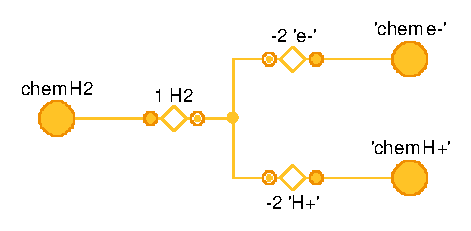
\includegraphics[width=0.5\linewidth]{4-HORD}}
    \label{fig:HOR}
  }\quad
  \subfloat[ORR ($4\timessep\s{e-} + 4\timessep\s{H+} + \s{O2} \rightarrow 2\timessep\s{H2O}$)]{
    \fbox{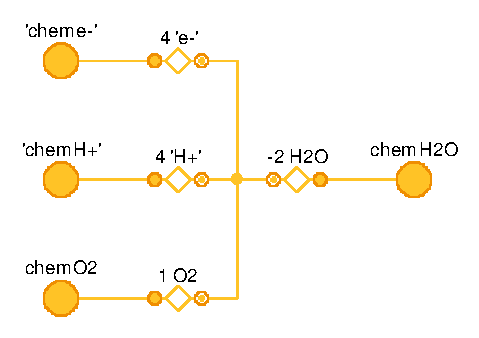
\includegraphics[width=0.5\linewidth]{4-ORRD}}
    \label{fig:ORR}
  }
  \caption{Diagrams of the reaction models}
  \label{fig:Reactions}
\end{figure}
 

\subsection{Electron Transfer and Charge Storage}

The \modelica{ElectronTransfer} model implements the Butler-Volmer equation (\ref{eq:Reaction}).  It includes advection and heat generation.  The heat is rejected to an \modelica{Inert} connector which is connected to the substrate (\n{C+}).  The Nernst equation is not implemented in this model (or any other model in the library) because the open circuit voltage is inherent in the properties of the species and their interconnection.

The \modelica{DoubleLayer} model stores and releases energy due to charge displacement across the electrolytic double layer.  Even though it is instantiated in the \modelica{graphite} phase (\autoref{sec:Phases}), it has its own volume (although small) which is introduced through an \modelica{Amagat} connector.  The  \modelica{DoubleLayer} model also has an \modelica{Inert} connector for translational and thermal exchange.  The electrons exit with either the velocity of that connector (typically zero) or the arrival velocity.  The first option, which is the default, implies that heat is generated; it is rejected through the same connector.  

The Modelica code and a table of parameters for \modelica{ElectronTransfer} and \modelica{DoubleLayer} are included in Sections~\ref{sec:FCSys_Chemistry_Electrochemistry_ElectronTransfer} and \ref{sec:FCSys_Chemistry_Electrochemistry_DoubleLayer}.


\subsection{Capillary Pressure}

Surface tension and capillary action are essential to remove liquid water from the cell.  The \modelica{Capillary} model applies capillary pressure between two \modelica{Amagat} connectors according to the Young-Laplace equation~\cite{Butt2003}.  It is instantiated within the \modelica{CapillaryVolume} model, where it yields a pressure difference between the liquid and the gas.  Since the water vapor is modeled as an ideal gas and the liquid has constant volume, the pressure difference shifts the saturation pressure according to the Kelvin equation~\cite{Butt2003}.

The Modelica code and a table of parameters for the \modelica{Capillary} model is included in \autoref{sec:FCSys_Chemistry_Capillary}.


\FloatBarrier % Flush the floats.
\section{Phases}
\label{sec:Phases}

\begin{contextbox}
  Related sections of the documentation:
  \vspace{0.5\baselineskip}

  \renewcommand{\arraystretch}{1.5}
  \begin{tabular}{ll}
    \docrow{sec:FCSys_Phases_PartialPhase}{FCSys.Subregions.Phases.PartialPhase}
  \end{tabular}
\end{contextbox}

There are four phase models---one for gas, one for liquid, and two different solids.  The \modelica{Gas} model contains \n{H2}, \n{H2O}, \n{N2}, and \n{O2}.  \modelica{Liquid} contains \n{H2O}.  \modelica{Graphite} contains \n{C+} and \n{e-}; \modelica{Ionomer} contains \n{H+}, \n{H2O}, and \s{SO3-} (abbreviation for \s{C19HF37O5S-}).  The species are conditionally included so that the \modelica{Gas} model can be used in both the anode (with \n{N2} and \n{O2} removed) and the cathode (with \n{H2} removed).

Within a phase, the species are combined according to Dalton's law.  The species exert forces on each other and exchange heat according to the diffusive exchange equations (\ref{eq:TranslationalDiffusiveExchange} and \ref{eq:ThermalDiffusiveExchange}).  By setting the independence factors to zero, it is possible to impose the assumption that the temperature or any component of velocity is equal among the species.  This causes the translation tool to simplify the model via index reduction.  
% Assuming the two phase flow of \n{FC} channel can be characterized as slug flow, the \n{VOF} method is appropriate (one set of momentum equations for all phases within each region) \cite[Ch. 23]{Fluent6.3}.

\autoref{fig:Phases} shows the diagrams of the phases.  All the phases have boundary bus connectors (\modelica{xNegative}, \modelica{xPositive}, etc.) to connect to adjacent subregions.  Species are labeled by their chemical formula when they are connected to the bus.  Each phase also has an \modelica{amagatDalton} adapter between Dalton's law (which is applied within the phase) and Amagat's law, which is applied among phases via the \modelica{amagat} connector.  The phases have \modelica{inter} connectors for inter-phase translational and thermal exchange.  Internal nodes (e.g., \modelica{commonExch}) are included as required for translational and thermal exchange within each phase.  Finally, the phases have chemical connectors (e.g., \modelica{chemH2O}) for chemical reactions and phase change among the phases.  The graphite phase (\autoref{fig:Graphite}) has a model for electron transfer (\modelica{electronTransfer}) and an optional electrolytic double layer capacitance (\modelica{doubleLayer}). 

\begin{figure}[htbp]
  \subfloat[Gas]{
    \fbox{\lwincludegraphics[width=0.82\linewidth]{4-Phases-GasD}}
    \label{fig:Gas}
  }\quad
  \subfloat[Graphite]{
    \fbox{\lwincludegraphics[width=8cm]{4-Phases-GraphiteD}}
    \label{fig:Graphite}
  }\quad
  \subfloat[Liquid]{
    \fbox{\lwincludegraphics[height=5cm]{4-Phases-LiquidD}}
    \label{fig:Liquid}
  }
  \phantomcaption
\end{figure}

\begin{figure}[htb]
  \ContinuedFloat
  \subfloat[Ionomer]{
    \fbox{\lwincludegraphics[width=10.2cm]{4-Phases-IonomerD}}
    \label{fig:Ionomer}
  }
  \caption{Diagrams of the phases}
  \label{fig:Phases}
\end{figure}


\autoref{fig:PhaseGUI} shows the parameter dialog for the gas phase.  The species can be enabled or disabled and their settings can be changed by opening the sub-dialogs shown in \autoref{fig:SpeciesGUI}.

\begin{figure}[htbp]
  \gui{4-GUI-Gas-General}
  \caption{Parameter dialog for the gas phase}
  \label{fig:PhaseGUI}
\end{figure}


\FloatBarrier % Flush the floats.
\section{Subregions}
\label{sec:Subregions}

\begin{contextbox}
  Related sections of the documentation:
  \vspace{0.5\baselineskip}

  \renewcommand{\arraystretch}{1.5}
  \begin{tabular}{ll}
    \docrow{sec:FCSys_Subregions_Subregion}{FCSys.Subregions.Subregion}
  \end{tabular}
\end{contextbox} 

The smallest unit of spatial discretization is the \modelica{Subregion} model, which is shown in \autoref{fig:Subregion}.  It contains instances of the phase models---\modelica{liquid}, \modelica{gas}, \modelica{graphite}, and \modelica{ionomer}.  They are connected to the \modelica{volume} model, which imposes the total volume of the subregion and applies capillary pressure between the gas and the liquid (see \autoref{sec:Chemistry}).  All of the phases are connected to the internal \modelica{commonExch} node for translational and thermal exchange.  The gas and liquid have an additional means of diffusive exchange via the \modelica{gasLiq} node.  Although not shown in the diagram, the chemical connectors of the phases are connected to the chemical reactions (\modelica{HOR} and \modelica{ORR}) described in \autoref{sec:Chemistry}.  The chemical connectors are directly connected for phase change---between gas and liquid and between gas and the ionomer (also not shown in the diagram). 

\begin{figure}[htbp]
  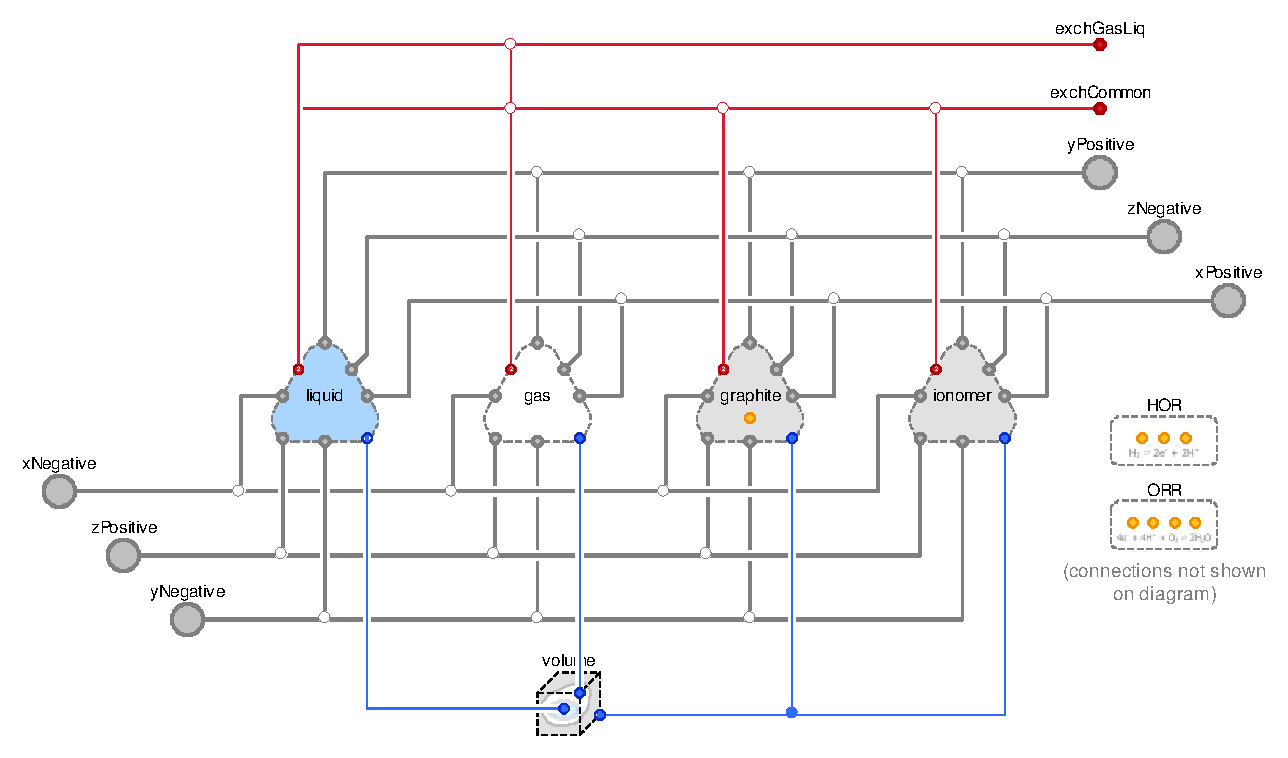
\includegraphics[width=\linewidth]{4-SubregionD}%
  \caption{Diagram of a subregion}
  \label{fig:Subregion}
\end{figure}

The external connectors (\modelica{xNegative}, \modelica{xPositive}, etc.) represent the boundaries of the rectilinear control volume.   Phases are labeled (\modelica{gas}, \modelica{liquid}, etc.) when they are connected to the boundaries.  By default, the \modelica{Subregion} model is \n{3D}.  However, assumptions may be applied via the Boolean parameters shown in \autoref{fig:SubregionGUIAssumptions} (and listed in \autoref{tab:FCSys_Subregions_Subregion-params}) to individually eliminate components of translational momentum and pairs of boundary connectors.  The settings for the phases (\autoref{fig:PhaseGUI}) can be accessed through the main tab of the parameter dialog shown in \autoref{fig:SubregionGUIGeneral}.

\begin{figure}[htbp]
  \subfloat[General parameters]{
    \gui{4-GUI-Subregion-General}
    \label{fig:SubregionGUIGeneral}
  }\quad
  \subfloat[Assumptions]{
    \gui{4-GUI-Subregion-Assumptions}
    \label{fig:SubregionGUIAssumptions}
  }
  \caption{Parameter dialog for a subregion}
  \label{fig:SubregionGUI}
\end{figure}


\FloatBarrier % Flush the floats.
\section{Regions\slash{}Layers}

\begin{contextbox}
  Related sections of the documentation:
  \vspace{0.5\baselineskip}

  \renewcommand{\arraystretch}{1.5}
  \begin{tabular}{ll}
    \docrow{sec:FCSys_Regions_AnCLs_AnCL}[sec:FCSys_Regions_Region]{FCSys.Regions.*}
  \end{tabular}
\end{contextbox}

 The layers of the cell are represented by regions which contain \n{3D} arrays of subregions.  Each layer is an extension of a base \modelica{Region} model with the appropriate settings (e.g., geometry and selection of species).   The grid is fixed and rectilinear but may have irregular spacing.  \autoref{fig:RegionImplemented} shows the diagram of the \modelica{Region} model.  The \modelica{subregions} icon in the center actually represents an array of subregions (which defaults to \num{1 x 1 x 1}).  The interconnections are automatically included.  \autoref{fig:RegionExpanded} shows the equivalent form for a \num{2 x 2 x 2} array, without the external connectors.  The boundaries (\modelica{xNegative}, \modelica{xPositive}, etc.) are \n{2D} arrays of bus connectors.


\begin{figure}[htbp]
  \subfloat[As implemented]{
    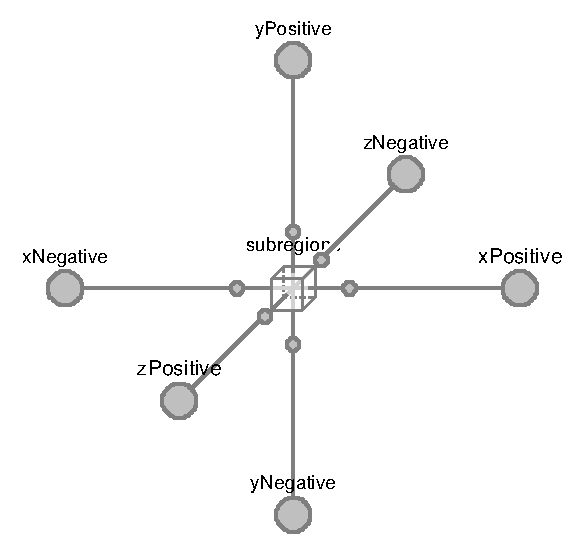
\includegraphics[width=0.46\linewidth]{4-RegionD}
    \label{fig:RegionImplemented}
  }\quad
  \subfloat[Expanded to show interconnections]{
    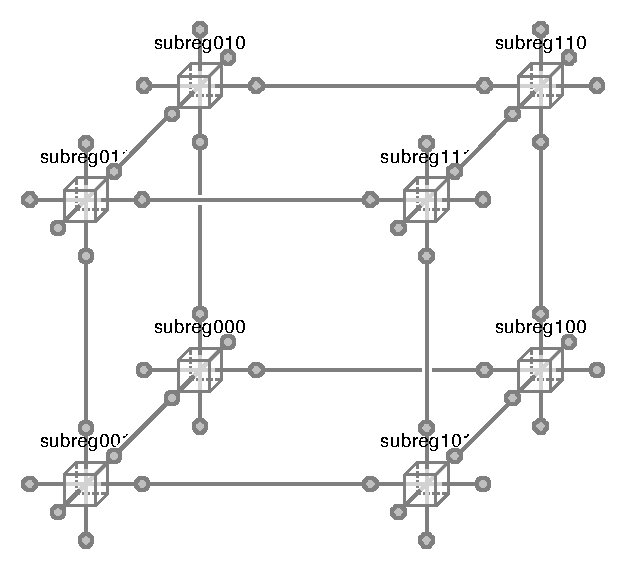
\includegraphics[width=0.46\linewidth]{4-MatrixD}
    \label{fig:RegionExpanded}
  }
  \caption{Diagrams of a region}
  \label{fig:Region}
\end{figure}


\autoref{fig:RegionGUI} shows the parameter dialog for a region model---the anode flow plate.  The lengths (\s{L}[_y], \s{L}[_y], and \s{L}[_z]) are one-dimensional arrays that contain the lengths of the subregions along the corresponding dimensions.  Only the z-axis boundaries are optional (\autoref{fig:RegionGUIAssumptions}) because the x- and y-axis boundaries are required due to the cell geometry.


\begin{figure}[htbp]
  \subfloat[General parameters]{
    \gui{4-GUI-AnFP-General}
    \label{fig:RegionGUIGeneral}
  }\quad
  \subfloat[Assumptions]{
    \gui{4-GUI-AnFP-Assumptions}
    \label{fig:RegionGUIAssumptions}
  }
  \caption{Parameter dialog for the anode flow plate}
  \label{fig:RegionGUI}
\end{figure}


\FloatBarrier % Flush the floats.
\section{Assemblies\slash{}Cells}


As shown in \autoref{fig:CellDiagrams}, the diagram of the fuel cell model (\autoref{fig:CellModel}) corresponds directly to the physical structure of the cell (\autoref{fig:Cell} and \autoref{fig:CellFlows}).  \autoref{fig:SimpleCellModel} shows a version of the cell model with nearly minimal complexity given the present modeling framework.  Its gas diffusion and catalyst layers are integrated (\modelica{anCGDL} and \modelica{anCGDL}) and all the species have the same temperature in every subregion, regardless of phase.

By default, each layer only contains one subregion (i.e., 1D model), but this can be increased.  The number of sets of subregions and the lengths of the subregions in the y and z directions (along and across the channel) are the same for all of the layers.  However, the number of sets of subregions and the lengths of the subregions are independent in the x direction (through the cell).


\begin{figure}[htbp]
  \subfloat[Physical structure]{
    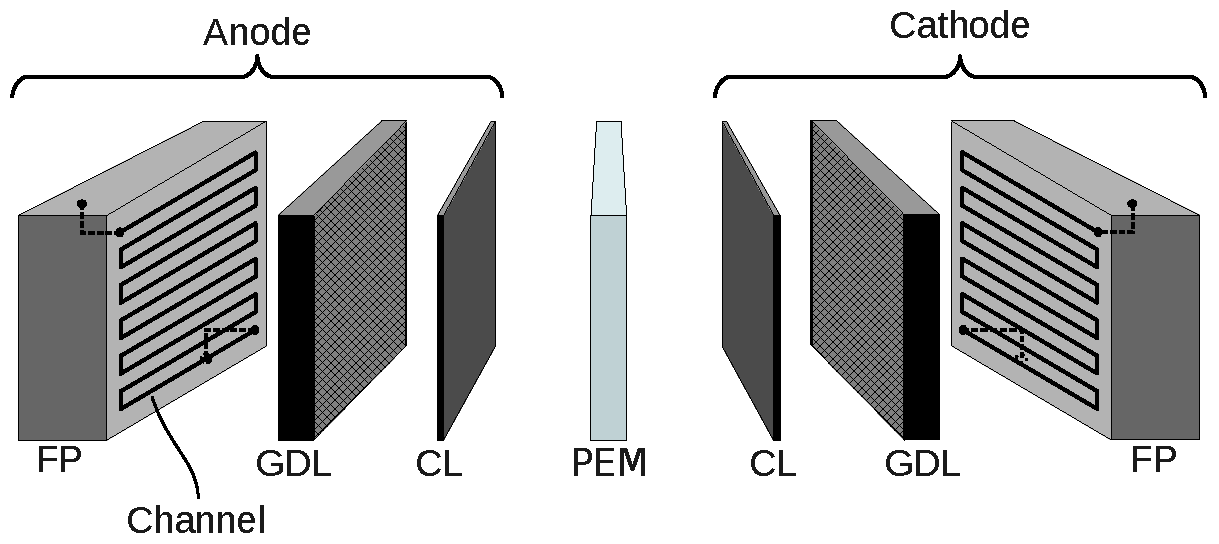
\includegraphics[width=0.75\linewidth]{1-Cell}
    \label{fig:Cell}
  }\quad
  \subfloat[Standard model diagram]{
    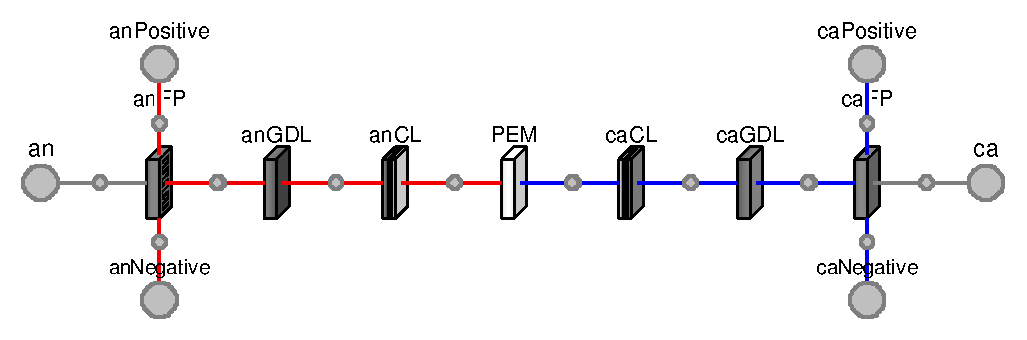
\includegraphics[height=5cm]{4-CellD}
    \label{fig:CellModel}
  }\quad
  \subfloat[Simplified model diagram]{
    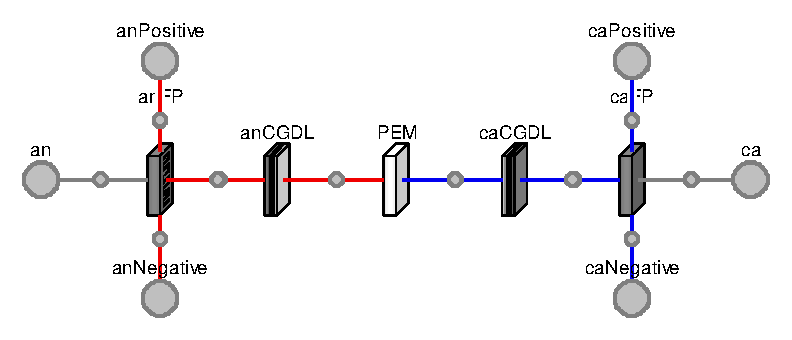
\includegraphics[height=5cm]{4-SimpleCellD}
    \label{fig:SimpleCellModel}
  }
  \caption{Single-cell \n{PEMFC}}
  \label{fig:CellDiagrams}
\end{figure}



\FloatBarrier % Flush the floats.
\section{Test Stand}
\label{sec:TestStand}

\begin{contextbox}
  Related section of the documentation:
  \vspace{0.5\baselineskip}

  \renewcommand{\arraystretch}{1.5}
  \begin{tabular}{ll}
    \docrow{sec:FCSys_Assemblies_Cells_Examples_TestConditions}[sec:FCSys_Assemblies_Cells_Examples_TestStand]{FCSys.Assemblies.Cells.Examples.*}
    \docrow{sec:FCSys_Conditions_Environment}{FCSys.Conditions.Environment}
  \end{tabular}
\end{contextbox}

The highest physical level of the library is the \modelica{TestStand} model, which applies boundary conditions to the fuel cell.  As shown in \autoref{fig:TestStandD}, there are four boundary conditions for the channels---a source and a sink for both the anode and cathode.  The cell model is bidirectional, so the choice of inlet and outlet can be switched via \modelica{anRouter} and \modelica{caRouter}.   By default, the \modelica{anBC} and \modelica{caBC} models apply uniform temperature to the exterior of the flow plates along the x axis.  An electrical model from the Modelica Standard Library~\cite{ModelicaSL3.2} is connected as a load to the first (1, 1) segment of the cell in the yz plane via the \modelica{anAdapt} and \modelica{caAdapt} adapters.  The default load is a current ramp (\modelica{Modelica.Electrical.Analog.Sources.CurrentRamp}).  

Besides the electrical load, the following key conditions are adjustable:
\begin{enumerate*}
  \item Temperature of the end plates and reactant sources
  \item Relative humidities of the reactant sources (independently adjustable)
  \item Fixed or stoichiometrically-varying reactant flow rates (independently adjustable)
  \item Fraction of \n{N2} in the cathode supply
  \item Pressures of the reactant sinks
  \item Optional inclusion of liquid water
\end{enumerate*}

\begin{figure}[htbp]
  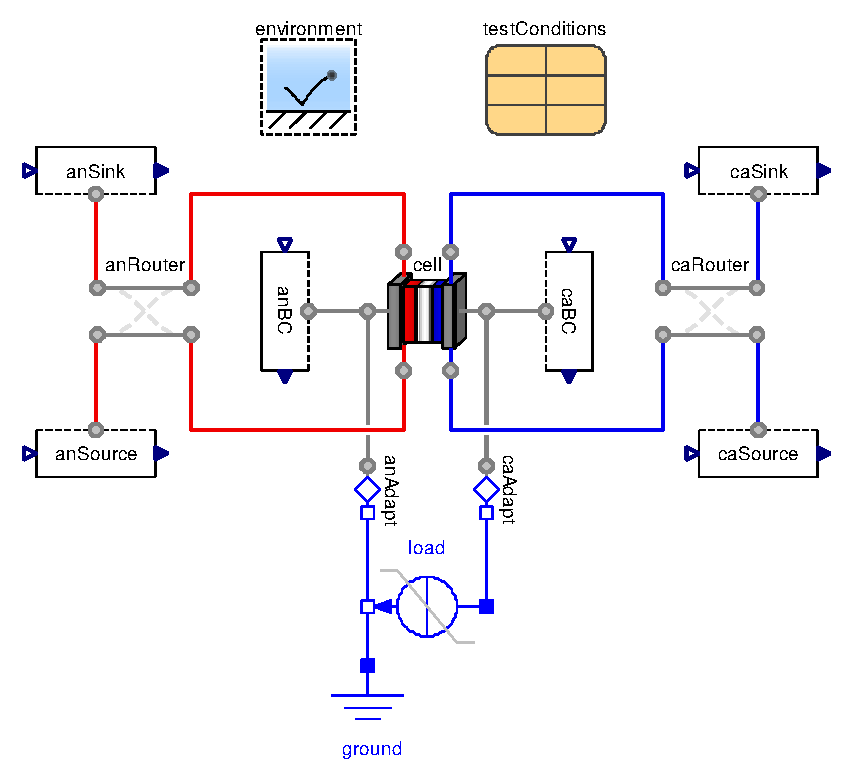
\includegraphics[width=0.8\linewidth]{4-TestStandD}%
  \caption{Diagram of the fuel cell test stand}%
  \label{fig:TestStandD}%
\end{figure}



\FloatBarrier % Flush the floats.
\section{Summary}

This chapter described the implementation of the model library in the Modelica language~\cite{Modelica3.3}.  It provided references to the more detailed documentation in \autoref{chap:Doc}.  The model library, like this chapter, builds from low-level classes such as types and constants to high-level classes such as the fuel cell model.  The models are highly modular and reconfigurable.  In the next chapter (\autoref{chap:Basic}), we will provide basic examples before exercising the full fuel cell model in \autoref{chap:Cell}.

